\documentclass{article}

\usepackage{latexsym}
\usepackage{graphicx}
\usepackage{amsmath}
\usepackage[fontset=mac]{ctex}
\usepackage{amsthm,amsmath,amssymb}
\usepackage{mathrsfs}
\usepackage{geometry}

\geometry{a4paper,scale=0.8}

\title{NumPDEs}
\author{欧阳尚可  3190102458}
\date{\today}

\begin{document}
\maketitle

\newpage
\section{Exercise}
\subsection{Ex 12.33}
\par 我们只验证$a\ge0$的情况,对于$a<0$的情况可以同理推出。由Taylor展开有
$$
u(x-h,t)=u-hu_x+\frac{1}{2}h^2u_{xx}-\frac{1}{6}h^3u_{xxx}+O(h^4)
$$
$$
u(x-2h,t)=u-2hu_x+2h^2u_{xx}-\frac{4}{3}h^3u_{xxx}+O(h^4) 
$$
$$
u(x,t+k)=u+ku_t+\frac{1}{2}k^2u_{tt}+\frac{1}{6}k^3u_{ttt}+O(k^3)
$$
代入得
$$
\tau(x,t)=\frac{u(x,t+k)-u(x,t)}{k}+\frac{a}{2h}(3u(x,t)-4u(x-h,t)+u(x-2h,t))-\frac{a^2k}{2h^2}(u(x,t)-2u(x-h,t)+u(x-2h,t))
$$
$$
=u_t+\frac{1}{2}ku_{tt}+\frac{1}{6}k^2u_{ttt}+O(k^3)+\frac{a}{2h}(2hu_x-\frac{2}{3}h^3u_{xxx})-\frac{a^k}{2h^2}(h^2u_{xx}-h^3u_{xxx})+O(h^2)=\frac{a^2kh}{2}u_{xxx}+O(h^2+k^2)
$$
注意到$k=O(h)$我们就可以得到方法在时间和空间上的二阶精确。

\subsection{Ex 12.34}
\par 要有$\textbf{U}^{n+1}=T\textbf{U}^n$,其中
$$
T = \textbf{I}-\frac{\mu}{2}
	\begin{bmatrix}
		3 &  &  & 1 & -4\\
		-4 & 3 & & & 1 \\
		1 & -4 & 3 & & \\
		& \ddots & \ddots & \ddots & \\
		& & 1 & -4 & 3 \\
	\end{bmatrix}
	+\frac{\mu^2}{2}
	\begin{bmatrix}
		1 &  &  & 1 & -2 \\
		-2 & 1 & & & 1 \\
		1 & -2 & 1 & & \\
		& \ddots & \ddots & \ddots & \\
		& & 1 & -2 & 1 \\
	\end{bmatrix}
$$
我们有T的特征向量$\omega^{p}$,其中$\omega^p_j=e^{2\pi ipjh},p,j=1,2,...,m+1$
$$
(M\omega^p)_j=(1-\frac{\mu}{2}(3-4e^{-2\pi iph}+e^{-4\pi iph})+\frac{\mu^2}{2}(1-2e^{-2\pi iph}+e^{-4\pi iph}))\omega^p_j
$$
因此我们有相应的特征值$\lambda_p=1-\frac{\mu}{2}(3-4e^{-2\pi iph}+e^{-4\pi iph})+\frac{\mu^2}{2}(1-2e^{-2\pi iph}+e^{-4\pi iph})=\frac{\mu^2-3\mu+2}{2}+\frac{\mu^2-\mu}{2}e^{-4\pi iph}+(2\mu-\mu^2)e^{-2\pi iph}$。进一步我们有
$$
\vert \lambda_p\vert^2=1+\mu(\mu-2)(\mu-1)^2sin^4(2\pi ph)
$$
要使得$\vert \lambda_p\vert\le1\Rightarrow \mu\in[0,2]$。\\

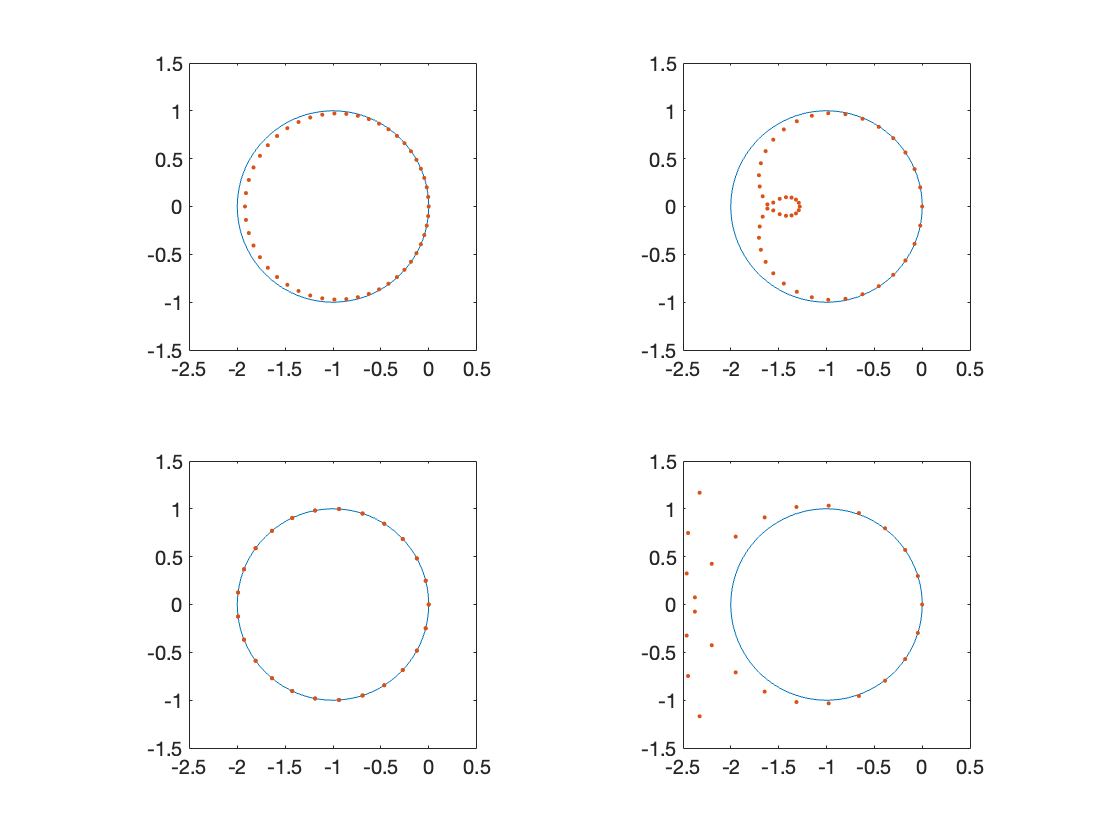
\includegraphics[scale=0.45]{Ex34.png}

\subsection{Ex 12.38}
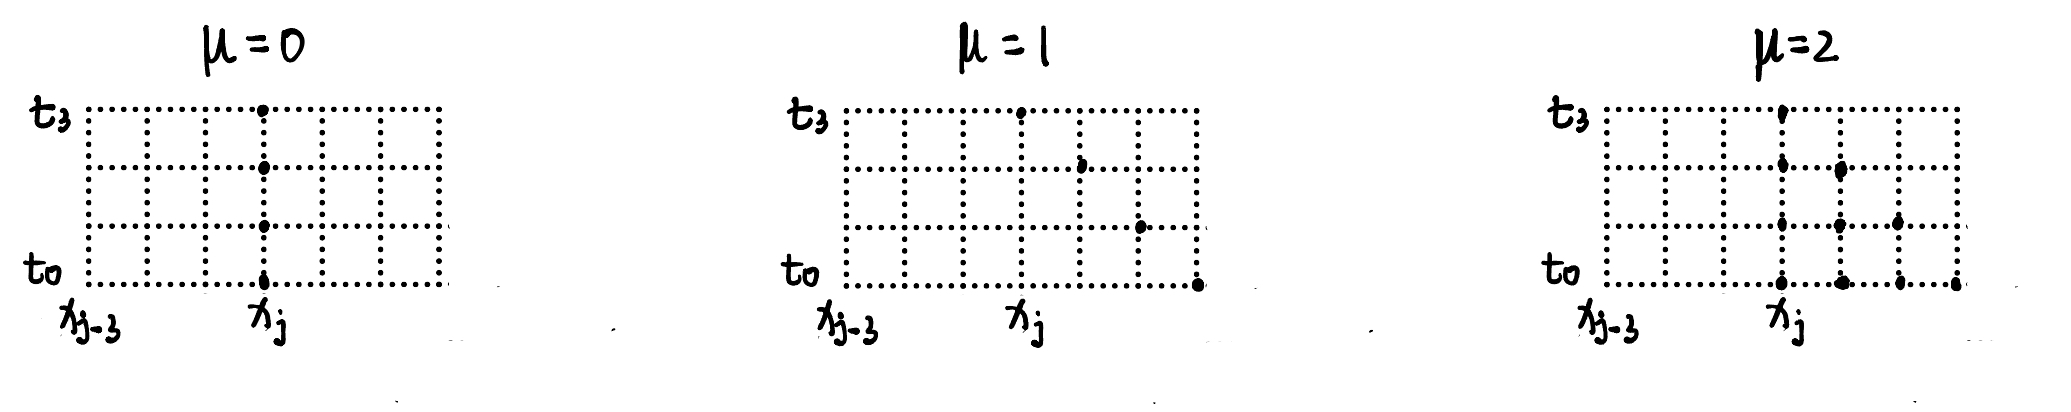
\includegraphics[scale=0.25]{Ex38.png}

\subsection{Ex 12.40}
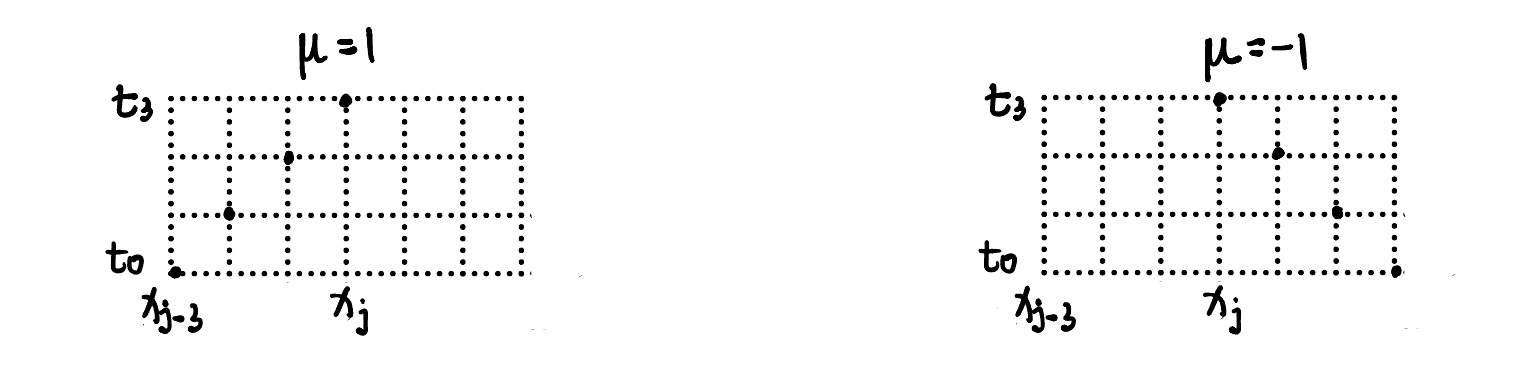
\includegraphics[scale=0.25]{Ex40.png}

\subsection{Ex 12.49}
\par 用$U_j^n=v(x,t)$我们有,同时令$h=O(k)$
$$
\frac{v(x,t+k)-v(x,t-k)}{2k}=a\frac{v(x+h,t)-v(x-h,t)}{2h}\Rightarrow v_t+av_x=-\frac{1}{6}k^2v_{ttt}-\frac{a}{6}h^2v_{xxx}+O(h^3)
$$
由上面的等式求偏导我们可以进一步得到
$$
v_{ttt}=-av_{xtt}+O(k); v_{ttx}=-av_{xxt}+O(k); v_{txx}=-av_{xxx}+O(k)
$$
代入得$v_t+av_x=\frac{a^3}{6}k^2v_{xxx}-\frac{a}{6}h^2v_{xxx}+O(k^3)\Rightarrow(12.43)$\\
\par 同理可得在$h=O(k)$时,有$v_t+av_x=-\frac{1}{6}k^2v_{ttt}-\frac{a}{6}h^2v_{xxx}-\frac{1}{120}k^4v_{ttttt}-\frac{1}{120}h^4v_{xxxxx}+O(k^6)$
由上面的等式求偏导我们可以进一步得到
$$
v_{ttt}=-av_{xtt}-\frac{1}{6}k^2v_{ttttt}-\frac{a}{6}h^2v_{xxxtt}+O(k^3);v_{xtt}=-av_{xxt}-\frac{1}{6}k^2v_{ttttx}-\frac{a}{6}h^2v_{xxxxt}+O(k^3)
$$
$$
v_{ttttt}=-av_{ttttx}+O(k);v_{ttttx}=-av_{tttxx}+O(k);v_{tttxx}=-av_{ttxxx}+O(k);v_{txxxx}=-av_{xxxxx}+O(k)
$$
代入化简可以得到$v_t+av_x+\frac{ah^2}{6}(1-\mu^2)v_{xxx}=\epsilon_fv_{xxxxx}$,其中$\epsilon_f=\frac{10a^3k^2h^2-9a^5k^4-h^4}{120}$。\\
\par 同理可以得到对于Lax-Wendroff有
$$
v_t+av_x+\frac{ah^2}{6}(1-\mu^2)v_{xxx}=\epsilon_wv_{xxxx}
$$

\subsection{Ex 12.50}
\par 用$U_j^n=v(x,t)$我们有,同时令$h=O(k)$
$$
\frac{v(x,t+k)-v(t,k)}{k}+\frac{a}{2h}(3v(x,t)-4v(x-h,t)+v(x-2h,t))=\frac{ka^2}{2h^2}(v(x,t)-2v(x-h,t)+v(x-2h,t))
$$
$$
\Rightarrow v_t+av_x=-\frac{1}{2}kv_{tt}+\frac{a^2}{2}kv_{xx}+\frac{a}{3}h^2v_{xxx}-\frac{a^2}{2}khv_{xxx}-\frac{1}{6}k^2v_{ttt}+O(k^3)
$$
由上面的等式求偏导我们可以进一步得到
$$
v_{tt}=-av_{xt}-\frac{1}{2}kv_{ttt}+\frac{a^2}{2}kv_{xxt}+O(k^2);v_{xt}=-av_{xx}-\frac{1}{2}kv_{xtt}+\frac{a^2}{2}kv_{xxx}+O(k^2)
$$
$$
v_{ttt}=-av_{ttx}+O(k);v_{ttx}=-av_{txx}+O(k);v_{txx}=-av_{xxx}+O(k)
$$
代入化简可以得到$v_t+av_x+\frac{ah^2}{6}(-2+3\mu-\mu^2)v_{xxx}$。\\
\par 在$\mu=0.8$的时候,$C_p$和$C_q$都是比$\vert a\vert$大的。

\subsection{Ex 12.51}
\par 在$\mu=1$的时候,对于两种方法而言都有$C_p$和$C_q$等于$a$。

\subsection{Ex 12.53}
\par 对于$U^n_j=[g(\xi)]^ne^{i\xi jh}$我们有
$$
g(\xi)=\frac{1-\mu}{2}e^{i\xi h}+\frac{1+\mu}{2}e^{-i\xi h}=cos(\xi h)-i\mu sin(\xi h)
$$
因此有$\vert g(\xi)\vert^2=cos^2(\xi h)+\mu^2sin(\xi h)$,由此得到$\vert g(\xi)\vert \le 1\Rightarrow \vert\mu\vert\le1$。

\subsection{Ex 12.54}
\par 对于$U^n_j=[g(\xi)]^ne^{i\xi jh}$我们有
$$
g(\xi)=1-\mu^2+\frac{\mu^2-\mu}{2}e^{i\xi h}+\frac{\mu^2+\mu}{2}e^{-i\xi h}=1-2\mu^2sin^2\frac{\xi h}{2}-i\mu sin(\xi h)
$$
因此有$\vert g(\xi)\vert^2=1-4\mu^2sin^2\frac{\xi h}{2}+4\mu^4sin^4\frac{\xi h}{2}+\mu^2sin^2(\xi h)$,由此得到$\vert g(\xi)\vert \le 1\Rightarrow \vert \mu \vert \le1$

\section{Programming}
对于$k=0.8h$\\
\includegraphics[scale = 0.175]{initial.png}
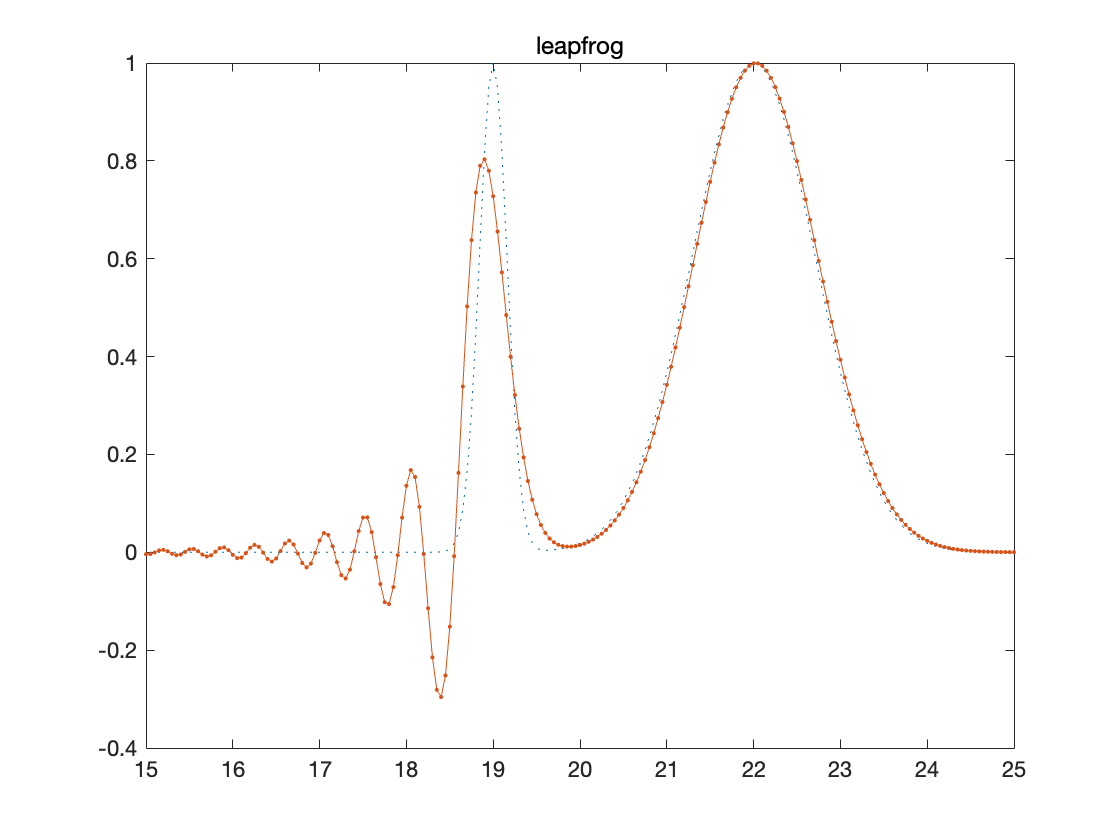
\includegraphics[scale = 0.175]{leapfrog.png}\\
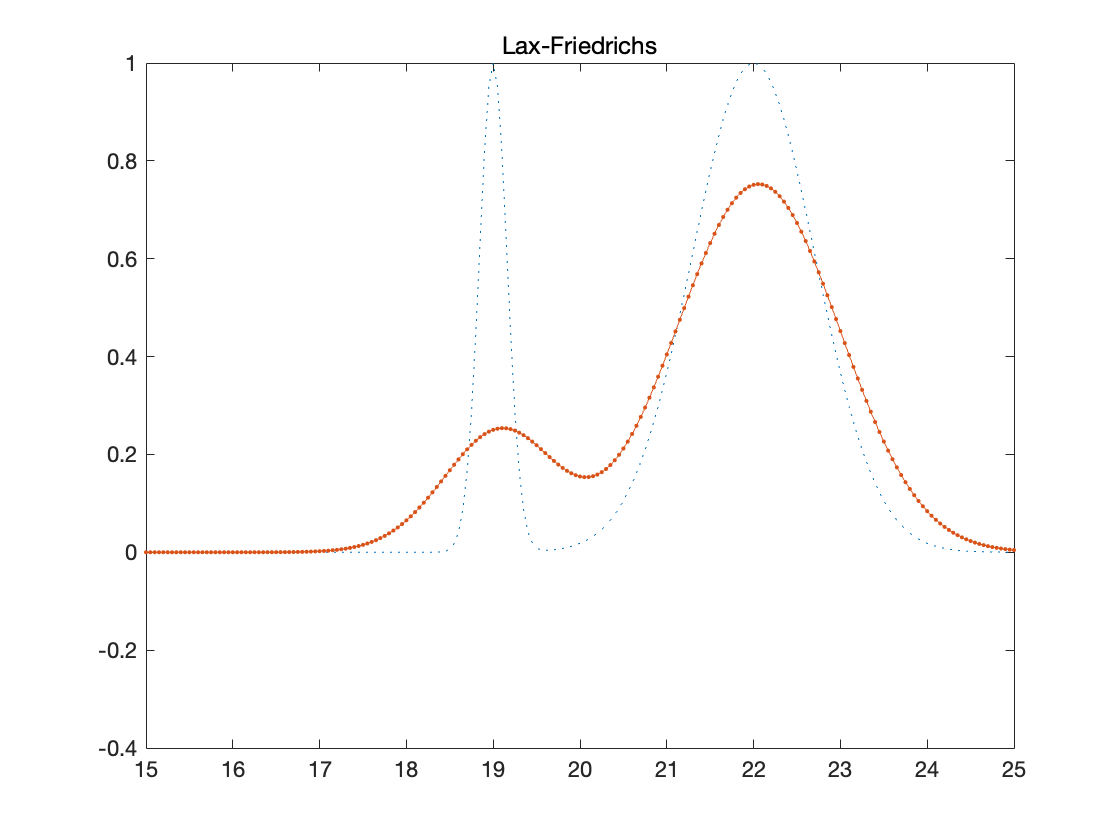
\includegraphics[scale = 0.175]{Lax_Friedrichs.png}
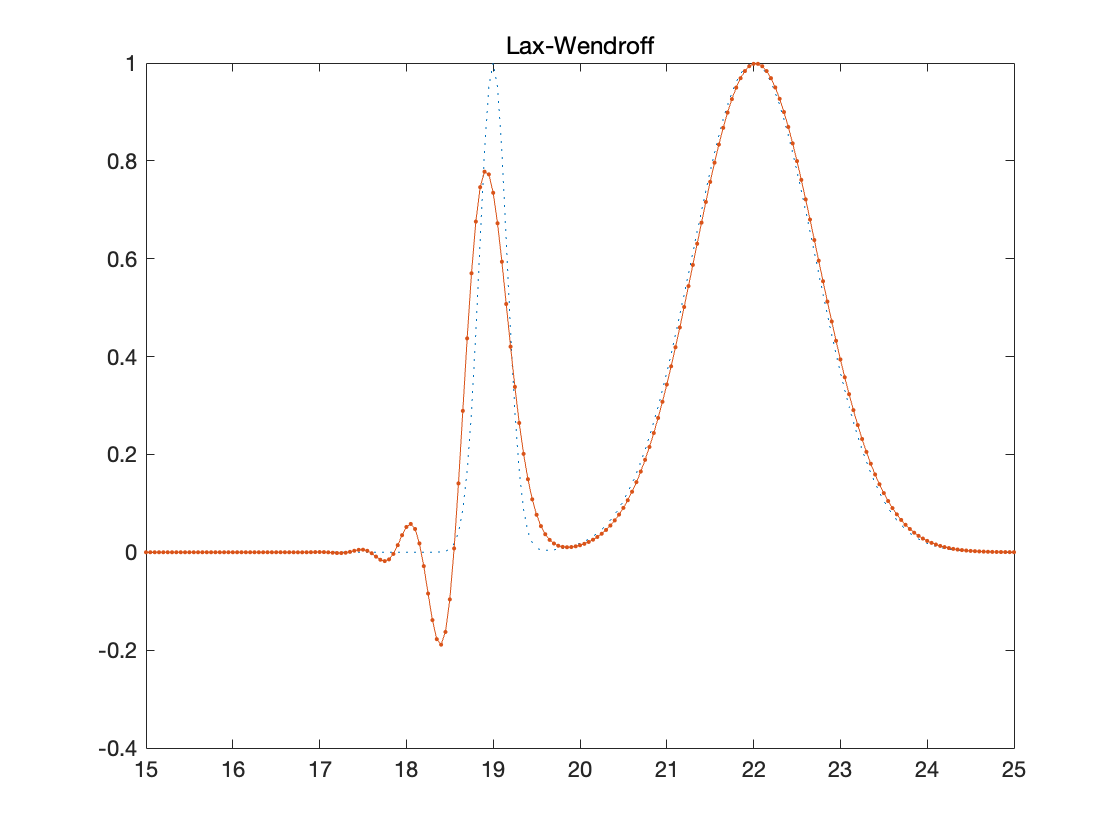
\includegraphics[scale = 0.175]{Lax_Wendroff.png}\\
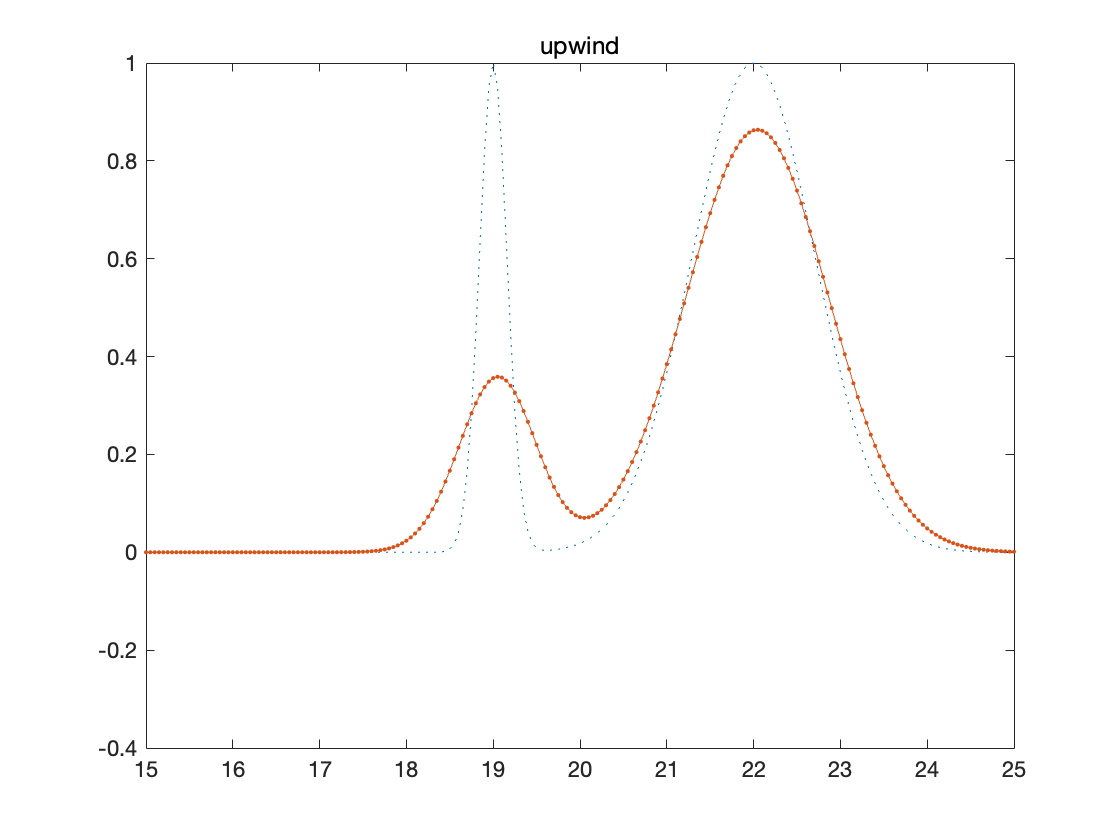
\includegraphics[scale = 0.175]{upwind.png}
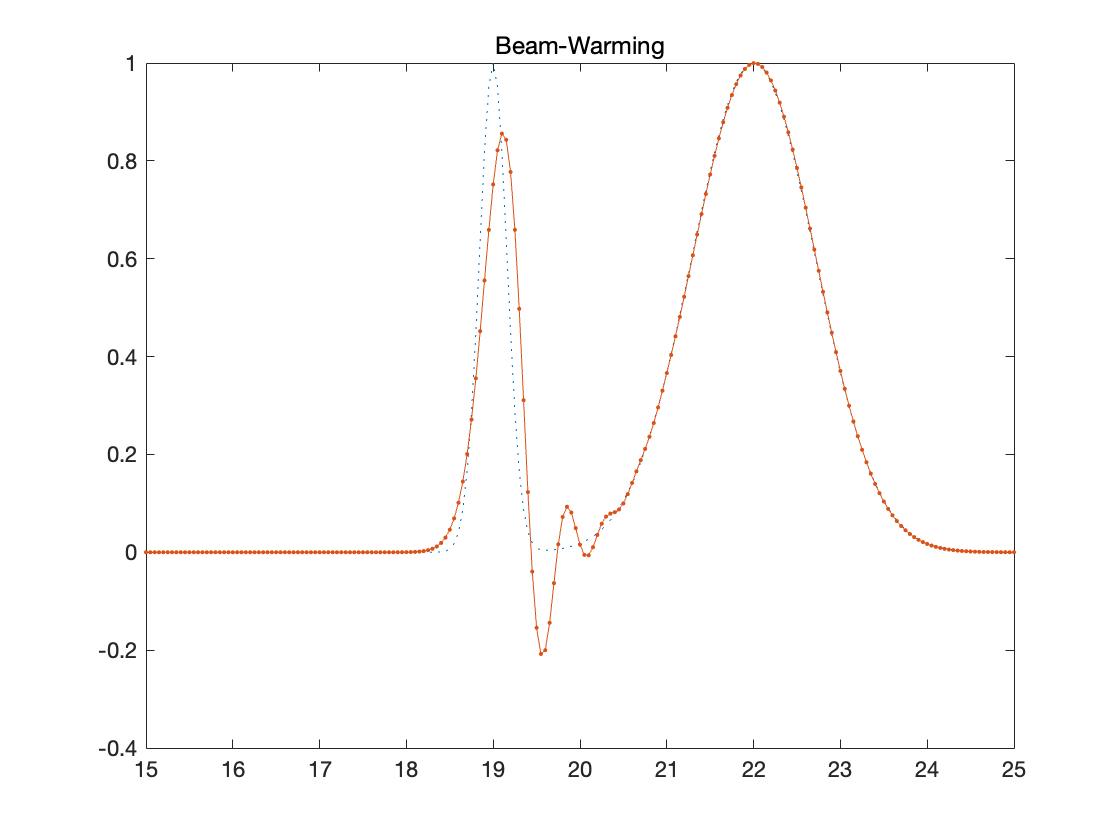
\includegraphics[scale = 0.175]{Beam_Warming.png}\\

对于$k=h$\\
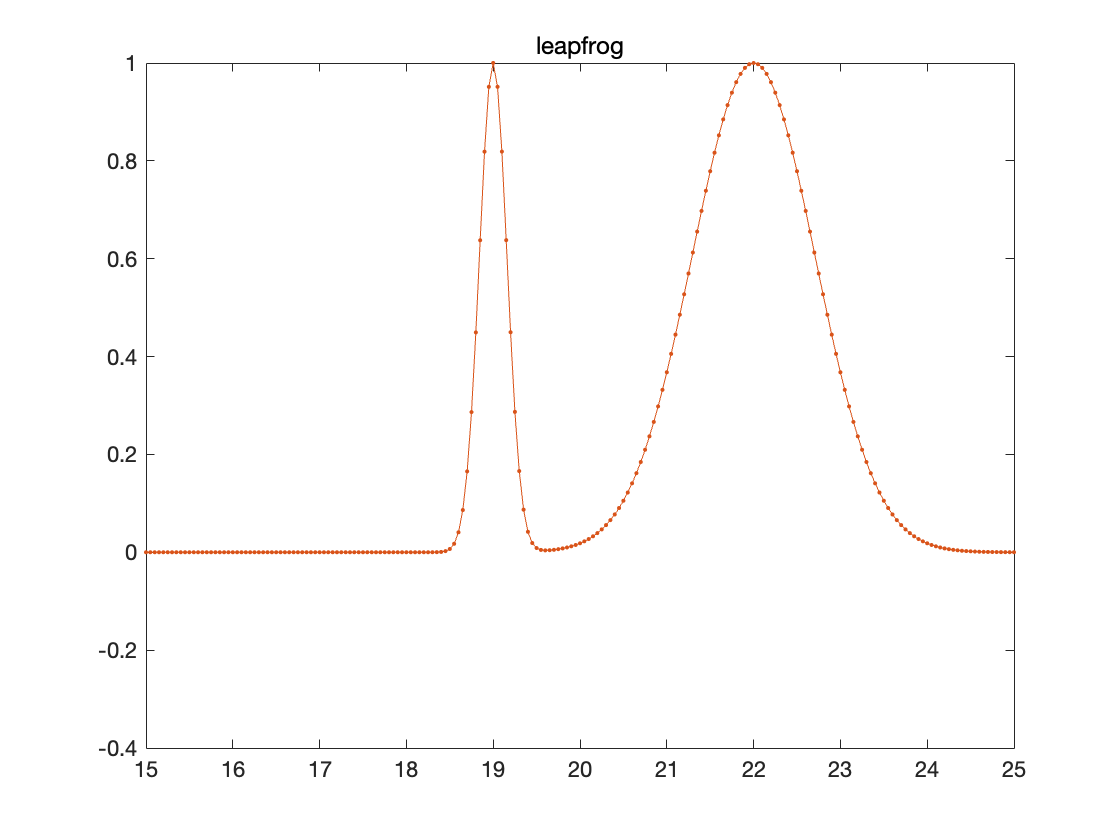
\includegraphics[scale = 0.175]{leapfrog1.png}
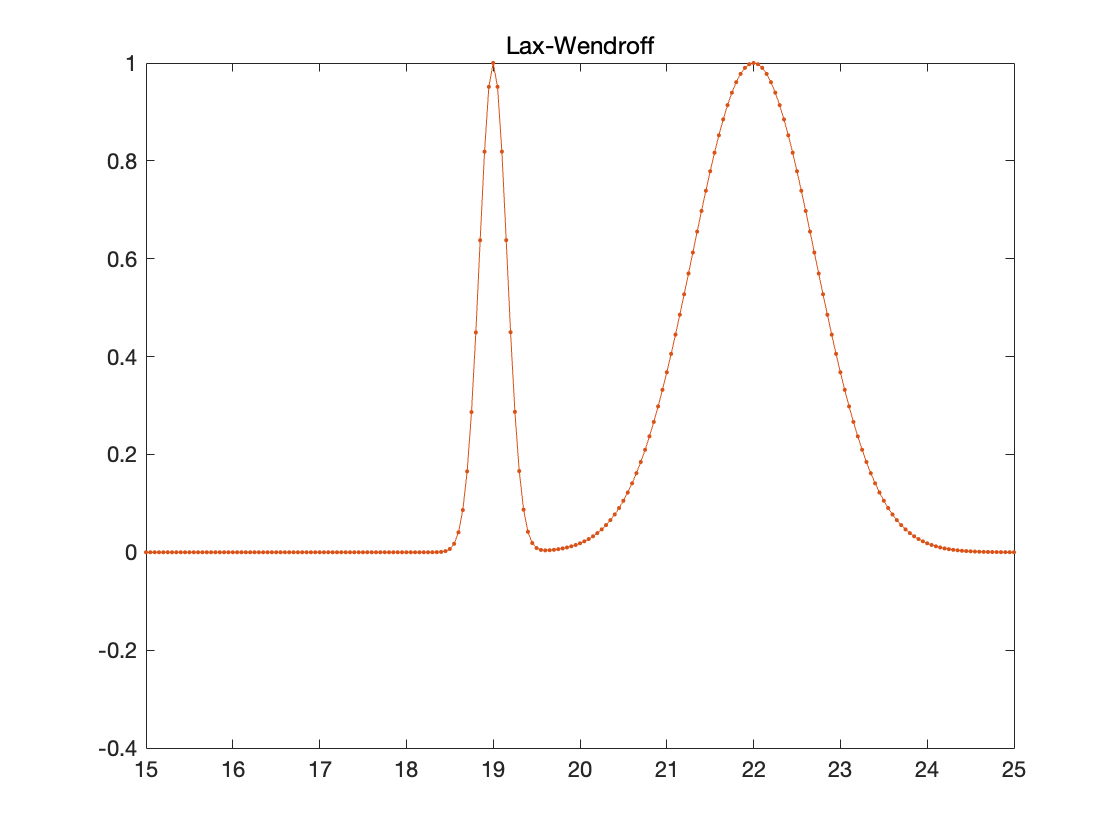
\includegraphics[scale = 0.175]{Lax_Wendroff1.png}




\end{document}